% !TeX encoding = UTF-8
\documentclass{sjtureport}
% !TEX root = ./main.tex

% pdf pages support
\usepackage{pdfpages}

% rotate text
\usepackage{lscape}

% Chemistry formulae support
\usepackage[version=4]{mhchem}

% Greek letters support
\usepackage{upgreek}

% Circuit drawing support
\usepackage{circuitikz}
% Add arrows for transistors
\ctikzset{tripoles/mos style=arrows}
\ctikzset{transistors/arrow pos=end}
% \coord: Show the position of nodes
\def\normalcoord(#1){coordinate(#1)}
\def\showcoord(#1){coordinate(#1) node[
			circle, red, draw, inner sep=1pt, pin={[red, overlay, inner sep=0.5pt, font=\tiny, pin distance=0.1cm, pin edge={red, overlay}]45:#1}](){}}
\let\coord=\normalcoord
\let\coord=\showcoord % Comment this line to hide coordinates

% 使用 BibLaTeX 处理参考文献
%   biblatex-gb7714-2015 常用选项
%     gbnamefmt=lowercase     姓名大小写由输入信息确定
%     gbpub=false             禁用出版信息缺失处理
\usepackage[backend=biber,style=gb7714-2015]{biblatex}
% 文献表字体
\renewcommand{\bibfont}{\zihao{5}\setbaselineskip{16bp}}
% 文献表条目间的间距
\setlength{\bibitemsep}{3bp plus 1pt}
% 导入参考文献数据库
\addbibresource{refs.bib}

% 脚注格式
\usepackage[perpage,bottom,hang]{footmisc}

% 定义图片文件目录与扩展名
\graphicspath{{figures/}}
\DeclareGraphicsExtensions{.pdf,.eps,.png,.jpg,.jpeg}

% 确定浮动对象的位置,可以使用 [H],强制将浮动对象放到这里(可能效果很差)
% \usepackage{float}

% 固定宽度的表格
% \usepackage{tabularx}

% 使用三线表:toprule,midrule,bottomrule。
\usepackage{booktabs}

% 表格中支持跨行
\usepackage{multirow}

% 表格中数字按小数点对齐
\usepackage{dcolumn}
\newcolumntype{d}[1]{D{.}{.}{#1}}

% 使用长表格
\usepackage{longtable}

% 附带脚注的表格
\usepackage{threeparttable}

% 附带脚注的长表格
\usepackage{threeparttablex}

% 算法环境宏包
\usepackage[ruled,vlined,linesnumbered]{algorithm2e}
% \usepackage{algorithm, algorithmicx, algpseudocode}

% 代码环境宏包
\usepackage{listings}
\lstdefinestyle{lstStyleCode}{%
  numbers           = left,
  breaklines        = true,
  aboveskip         = \medskipamount,
  belowskip         = \medskipamount,
  basicstyle        = \ttfamily\zihao{5},
  commentstyle      = \slshape\color{black!60},
  stringstyle       = \color{green!40!black!100},
  keywordstyle      = \bfseries\color{blue!50!black},
  extendedchars     = false,
  upquote           = true,
  tabsize           = 2,
  showstringspaces  = false,
  xleftmargin       = 1em,
  xrightmargin      = 1em,
  breaklines        = false,
  framexleftmargin  = 1em,
  framexrightmargin = 1em,
  backgroundcolor   = \color{gray!10},
  columns           = flexible,
  keepspaces        = true,
  texcl             = true,
  mathescape        = true
}
\lstnewenvironment{codeblock}[1][]{%
  \lstset{style=lstStyleCode,#1}}{}

% 直立体数学符号
\providecommand{\dd}{\mathop{}\!\mathrm{d}}
\providecommand{\ee}{\mathrm{e}}
\providecommand{\ii}{\mathrm{i}}
\providecommand{\jj}{\mathrm{j}}

% 国际单位制宏包
\usepackage{siunitx}
\sisetup{mode=match} % 与文本/数学环境字体匹配

% 定理环境宏包
\usepackage{amsthm}
% \usepackage{ntheorem}

% 绘图宏包
\usepackage{tikz}
\usetikzlibrary{arrows.meta, shapes.geometric}

% 数据图表宏包
\usepackage{pgfplots}
\pgfplotsset{compat=newest}

% 一些文档中用到的 logo
\usepackage{hologo}
\providecommand{\XeTeX}{\hologo{XeTeX}}
\providecommand{\BibLaTeX}{\textsc{Bib}\LaTeX}

% 借用 ltxdoc 里面的几个命令方便写文档
\DeclareRobustCommand\cs[1]{\texttt{\char`\\#1}}
\providecommand\pkg[1]{{\sffamily#1}}

% hyperref 宏包在最后调用
\usepackage{hyperref}

% E-mail
\providecommand{\email}[1]{\href{mailto:#1}{\urlstyle{tt}\nolinkurl{#1}}}


\begin{document}

%TC:ignore

% !TEX root = ./main.tex
\thispagestyle{empty}

\begin{titlepage}
	\begin{center}
		\includegraphics[width=\textwidth]{sjtu-vi-logo-red.pdf}
		\vspace*{1cm}

		\huge
		\textbf{本科课程项目报告} \\
		\Large
		\textbf{UNDERGRADUATE COURSE PROJECT REPORT}

		\vspace{2cm}
		\LARGE
		\textbf{HW2: 嵌入式系统开发} \\

		\vfill

		\large
		\begin{minipage}{0.2\textwidth}
			\begin{flushleft}
				\Large
				姓\qquad 名: \\
				学\qquad 号: \\
				课\qquad 程: \\
				任课教师: \\
				学院(系) : \\
				开课学期: 
			\end{flushleft}
		\end{minipage}
		~
		\begin{minipage}{0.7\textwidth}
			\begin{center}
				\Large
				Brian Li \\
				521030990021 \\
				MST4311-智能芯片与系统设计 \\
				刘婷 \\
				电子信息与电气工程学院 \\
				2024年 (秋季)
			\end{center}
		\end{minipage}
		
		%date
		\vspace{1cm}
		\Large
		\today
	\end{center}
\end{titlepage}


\tableofcontents

%TC:endignore

% 正文内容

\chapter{引言}

\section{实验目的}

\begin{itemize}
	\item 学会使用双通道 GPIO
	\item 学会使用中断
	\item 理解 IP 的设置和使用
	\item 实现简单的嵌入式系统的开发
\end{itemize}

\section{实验内容}

在 lab5 基础上,计数周期的计算改为 ONE\_TENTH * (2 bit SW + 2bit BTN)

\begin{itemize}
	\item \textbf{双通道 GPIO 设计}: 将 2 个 switch 按键 (SW0, 1) 和两个 button 按键 (BTN2, BTN3) 采用同一个 GPIO 接口挂在 AXI 总线上
	\item \textbf{中断程序设计}: 捕捉来自 PL BTN0 和 BTN1 的中断,使得按下按键0(1)时,通过 UART 串口输出 "Interrupt valid, Button 0(1) is pressed"
	\item \textbf{中断屏蔽设计}: 一次中断触发后,\SI{1}{\s} 内不响应第二次中断
\end{itemize}

本实验基于 Vivado 2018.2 实现。

\chapter{实验设计}

本实验的系统框图如图\ref{fig:block-design}所示。

\begin{figure}[!htp]
	\centering
	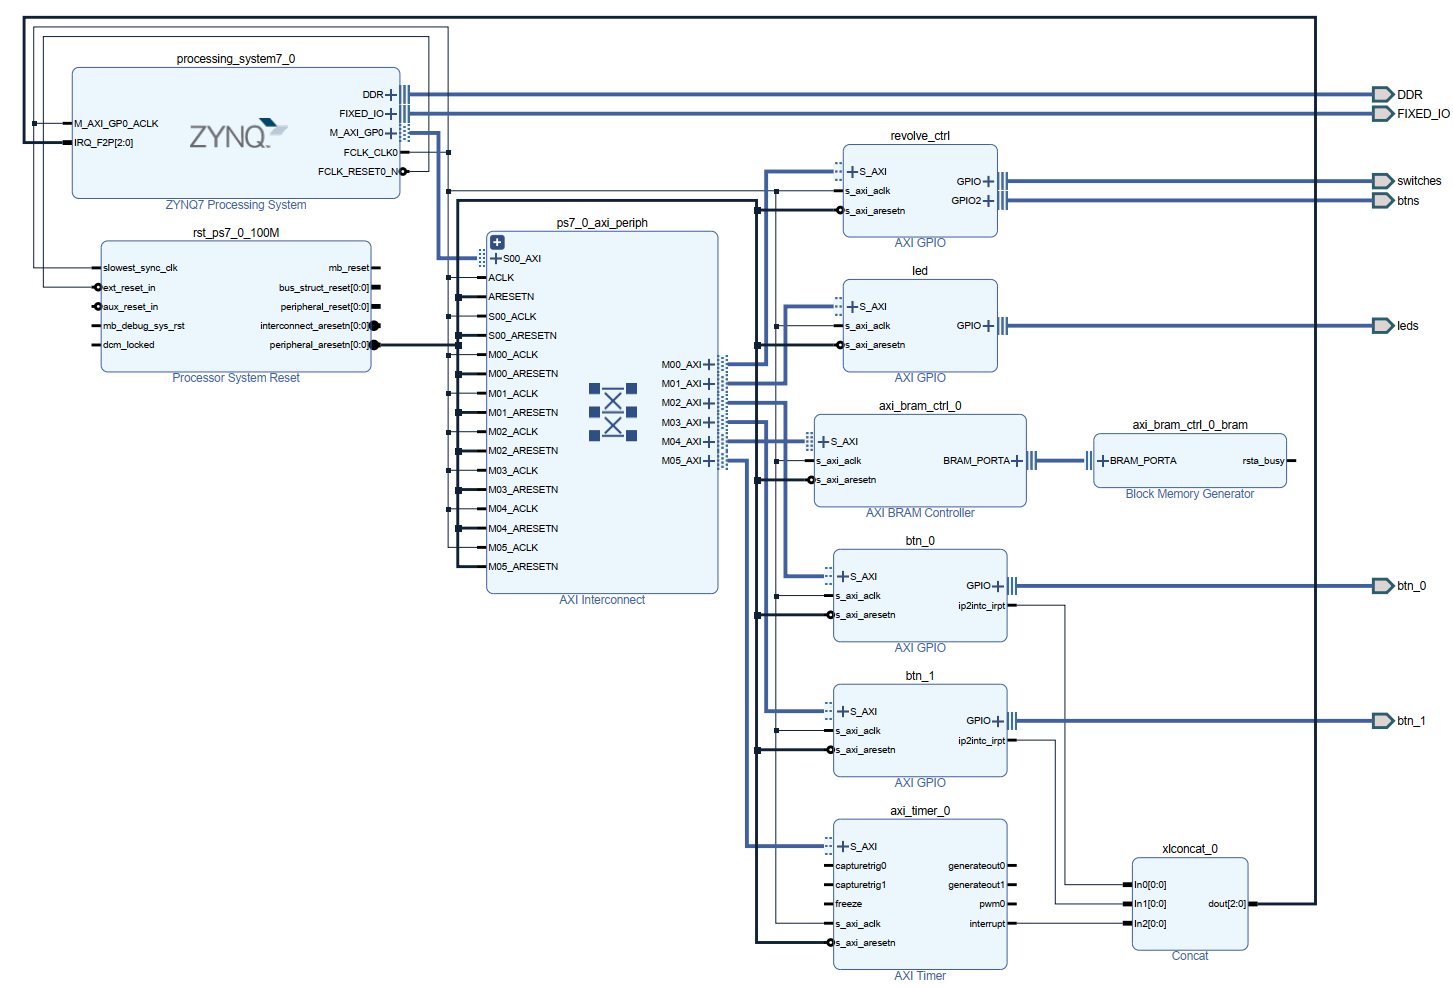
\includegraphics[width=\textwidth]{block_design}
	\caption{Block Design}
	\label{fig:block-design}
\end{figure}

考虑到实验要求中断的实现\textbf{尽量使用添加硬件管脚后利用软件驱动的方式},这里不添加 AXI Interrupt Controller,而是在 Zynq 核上添加 PL-PS 中断端口,后续通过编写 SDK 中的 .c 文件实现中断初始化、中断处理程序、中断屏蔽等。

图\ref{fig:block-design}中,按键 SWITCH 和 BUTTON 作为 AXI GPIO 的输入,LED 作为 AXI GPIO 的输出。在执行 lab5 跑马灯程序的同时,当 AXI GPIO 检测到按键0或1状态发生变化时,AXI GPIO 就会产生一个中断信号,直接传入 Zynq 核上的 PL-PS 中断端口,Zynq 核通过接收到的中断信号控制 UART 端口输出指定信息。

\section{Vivado 工程设计}

\subsection{Zynq 核}

创建一个空白 Zybo 工程,并新建 Block design。添加 IP: ZYNQ7 Processing System,执行 \textit{Run Block Automation},并按照 lab1 \textit{Configure the processing block with just UART 1 peripheral enabled} 节中的指导,去掉如下端口:

\begin{itemize}
	\item ENET
	\item USB 0
	\item SD 0
	\item GPIO MIO
	\item Quad SPI Flash
	\item Timer 0
\end{itemize}

之后如图\ref{fig:interrupt-port}所示,添加 PL-PS 中断端口。

\begin{figure}[!htp]
	\centering
	\begin{minipage}{0.48\textwidth}
		\centering
		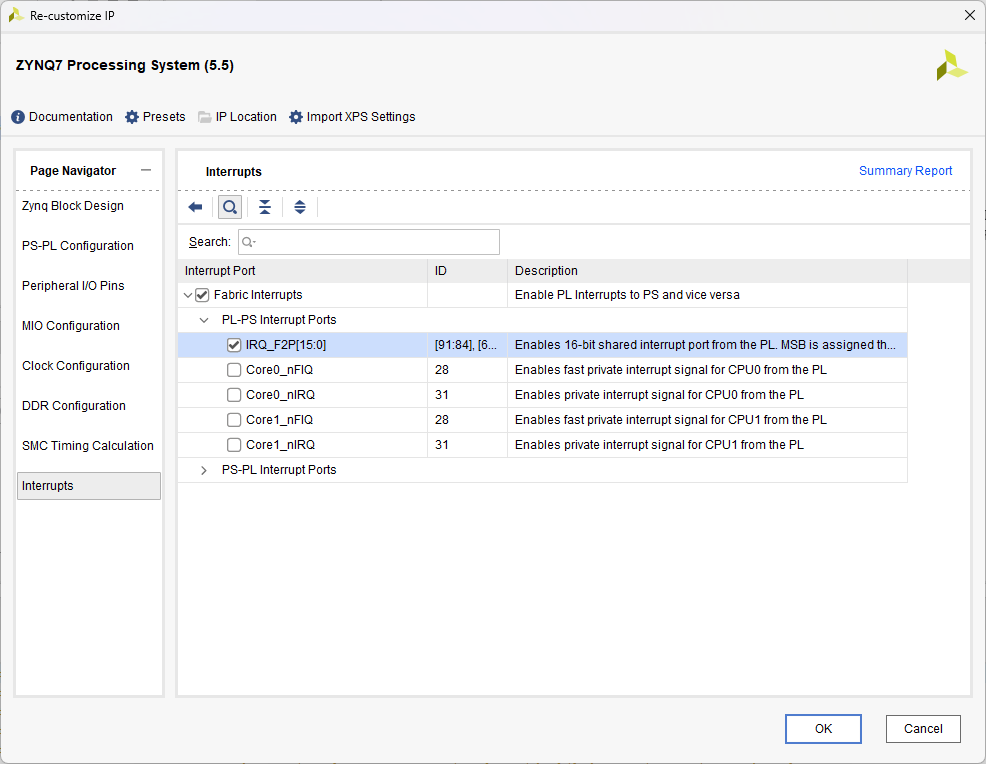
\includegraphics[width=\textwidth]{interrupt_port}
		\caption{PL-PS 中断端口设置}
		\label{fig:interrupt-port}
	\end{minipage}
	\begin{minipage}{0.48\textwidth}
		\centering
		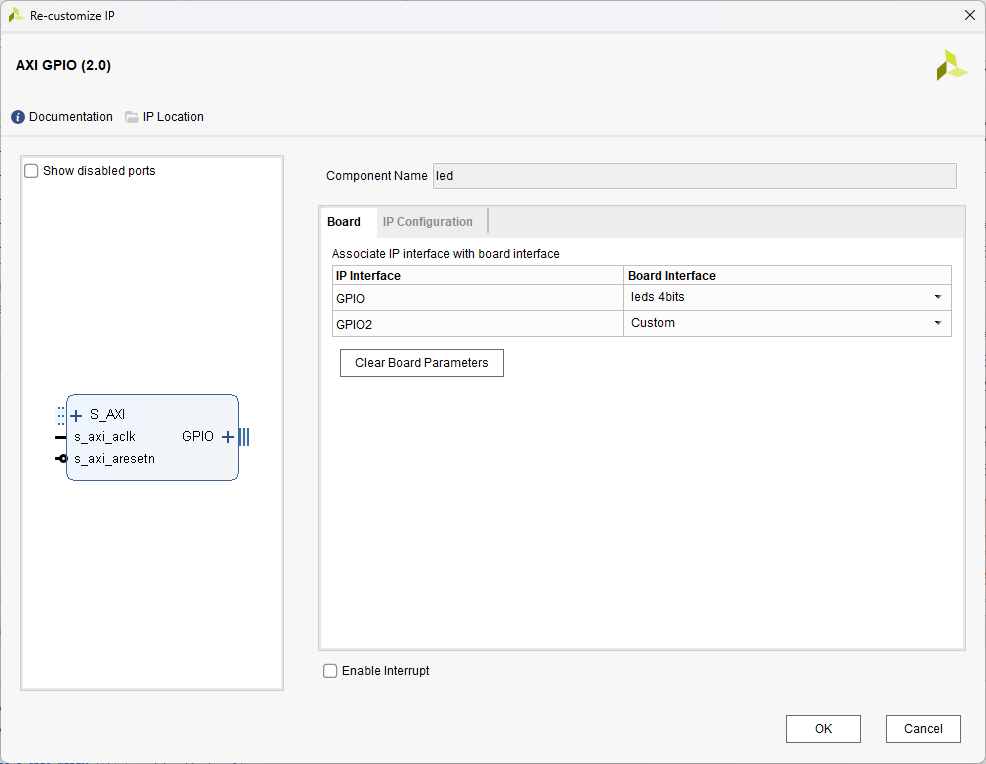
\includegraphics[width=\textwidth]{board_parameters_led}
		\caption{LED GPIO 端口设置}
		\label{fig:gpio-led}
	\end{minipage}
\end{figure}

\subsection{GPIO}

接下来添加 IP: AXI GPIO。共需要添加4个 AXI GPIO,分别用于 LED0-3 (走马灯),SW0-1 \& BTN2-3 (走马灯控制信号),BTN0 (生成中断),BTN1 (生成中断)。

如图\ref{fig:gpio-led}所示,设置 LED 的 AXI GPIO 端口。

如图\ref{fig:gpio-revolve-ctrl}所示,设置 SW0-3 和 BTN2-3 的 AXI GPIO 端口。该 GPIO 为双通道,通道一用于 SW0-3,通道二用于 BTN2-3。由于 BTN0 和 BTN1 需要另外用于产生中断,因此通道二不能设置为 btns\_4bit,需要先设置为 custom \SI{2}{\bit},后续在\ref{sec:io-planning}节设置管脚约束。

\begin{figure}[!htp]
	\centering
	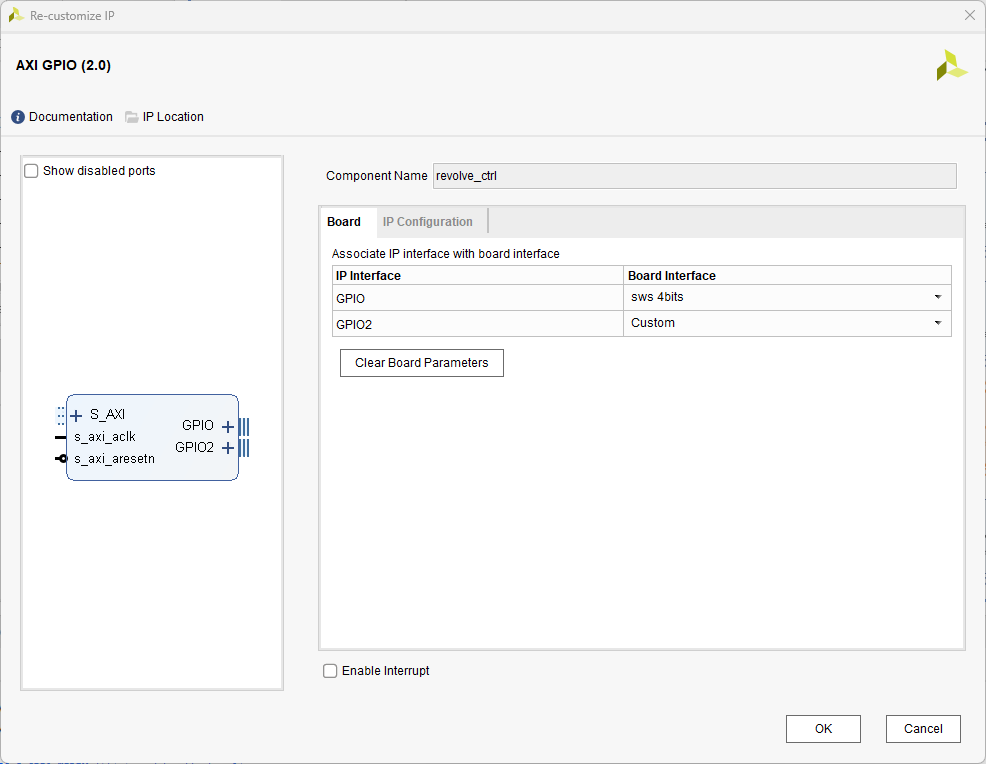
\includegraphics[width=0.48\textwidth]{board_parameters_revolve_ctrl}
	\hfill
	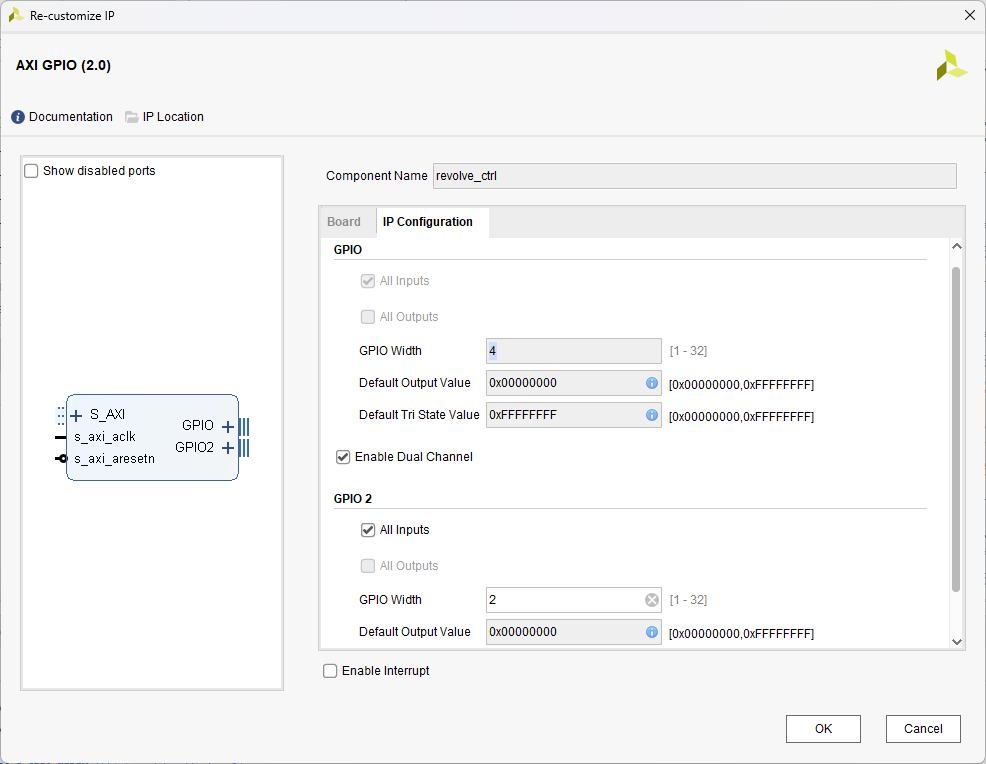
\includegraphics[width=0.48\textwidth]{ip_config_revolve_ctrl}
	\caption{SW0-3 和 BTN2-3 的 AXI GPIO 端口设置}
	\label{fig:gpio-revolve-ctrl}
\end{figure}

如图\ref{fig:gpio-btn0}所示,设置 BTN0,1 的\textbf{两个} AXI GPIO 端口。通道设置为 custom \SI{1}{\bit}。此处应勾选\textit{Generate Interrupt}以使该模块在 GPIO 信号改变时产生中断信号。

\begin{figure}[!htp]
	\centering
	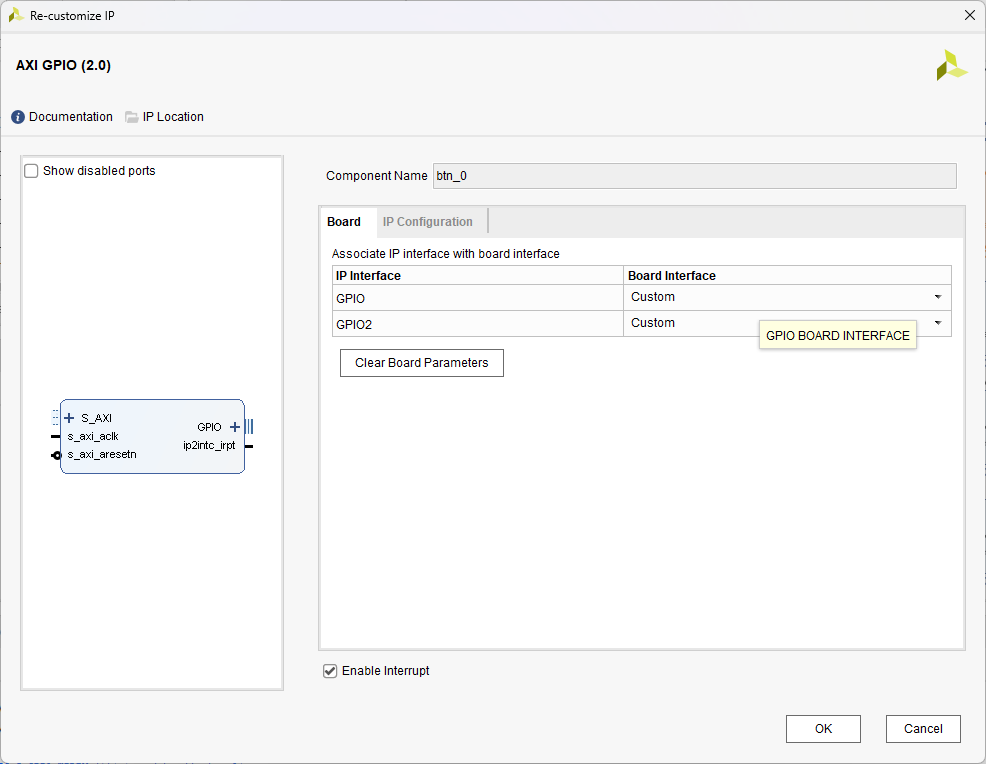
\includegraphics[width=0.48\textwidth]{board_parameters_btn0}
	\hfill
	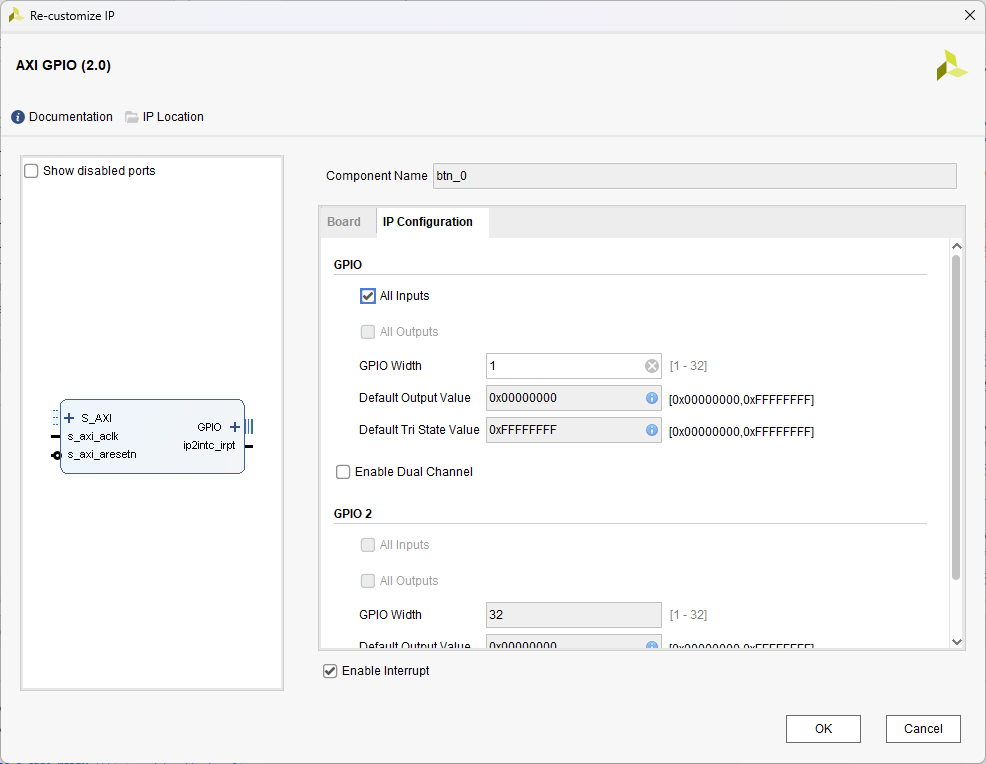
\includegraphics[width=0.48\textwidth]{ip_config_btn0}
	\caption{BTN0,1 的 AXI GPIO 端口设置}
	\label{fig:gpio-btn0}
\end{figure}

\subsection{其它 IP}

添加 IP: AXI Timer,用于为中断屏蔽提供定时器,如图\ref{fig:timer}所示。

\begin{figure}[!htp]
	\centering
	\begin{minipage}{0.48\textwidth}
		\centering
		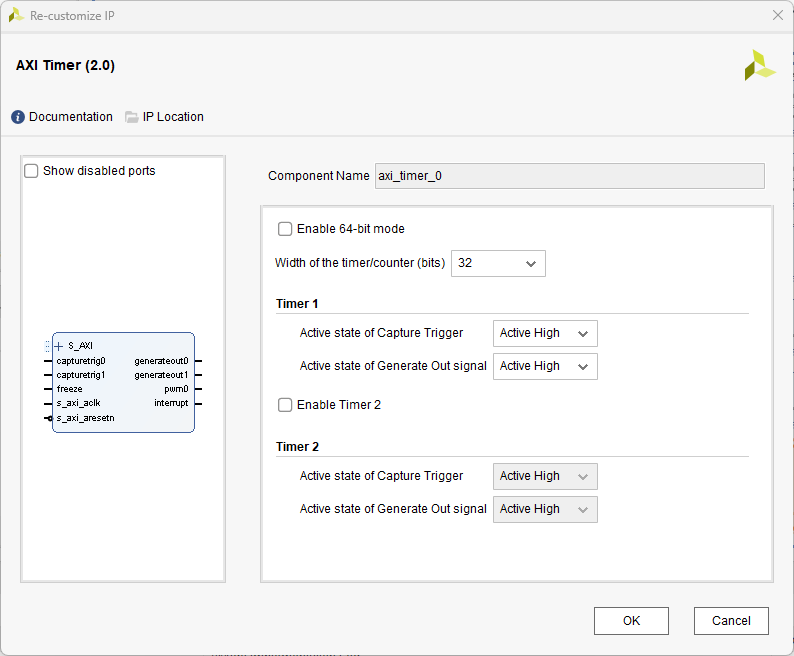
\includegraphics[width=\textwidth]{ip_config_timer.png}
		\caption{Timer IP 设置}
		\label{fig:timer}
	\end{minipage}
	\begin{minipage}{0.48\textwidth}
		\centering
		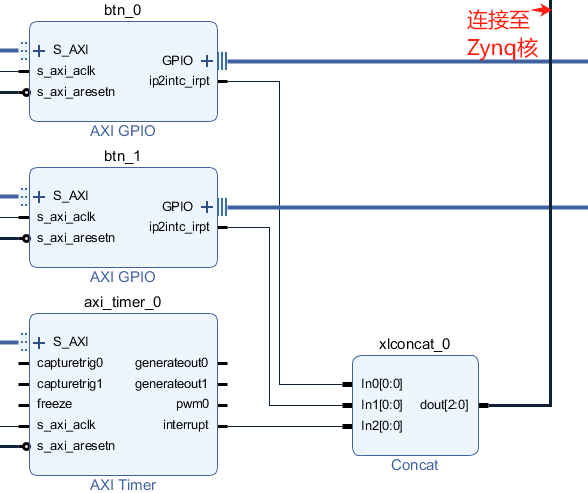
\includegraphics[width=\textwidth]{connection_concat}
		\caption{Concat 端口连线}
		\label{fig:concat}
	\end{minipage}
\end{figure}

添加 IP: Concat,用于将来自 BTN0,1,以及 AXI Timer 的中断信号组合为 \SI{3}{\bit} 的总线,并输出给 Zynq 核,如图\ref{fig:concat}所示。

\subsection{硬件综合}

点击 \textit{Run Connection Automation},完成连接,至此 Block design 设计完成, Block design 应如图\ref{fig:block-design}所示。之后,按照 lab1 \textit{Generate Top-Level and Export to SDK} 节中的指导,执行 \textit{Generate Output Products},生成 HDL Wrapper,并执行 \textit{Run Synthesis}。

\subsection{IO 规划}
\label{sec:io-planning}

打开 Synthesized Design,切换到 I/O Planning 视图,设置管脚约束。SW0-3 以及 LED0-3 的管脚已设置好,接下来设置 BTN0-3 的管脚约束,如图\ref{fig:io-planning}所示,将管脚约束保存为 .xdc 文件。

\begin{figure}[!htp]
	\centering
	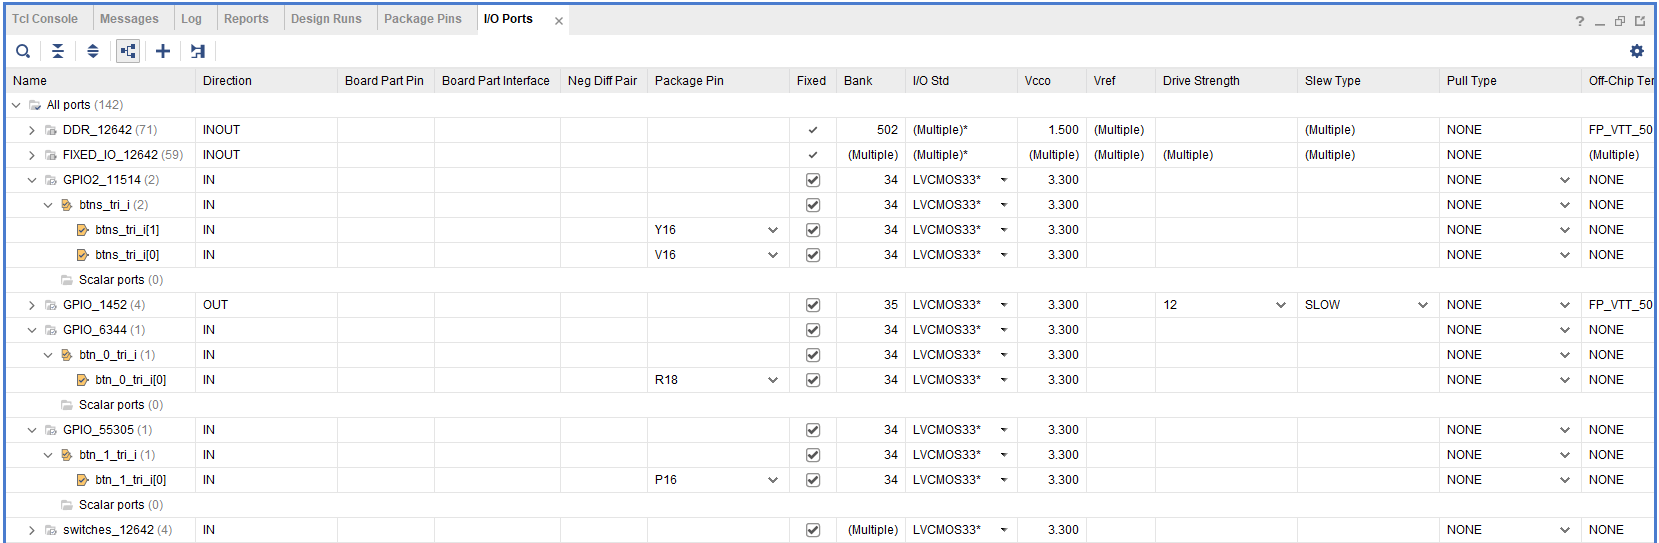
\includegraphics[width=\textwidth]{io_planning}
	\caption{BTN0-3 管脚约束设置}
	\label{fig:io-planning}
\end{figure}

\section{SDK 编程}

执行 \textit{Generate Bitstream}。在 Vivado 中点击 \textit{File -> Export -> Export Hardware},选择 \textit{Include Bitstream},点击 \textit{OK}。之后点击 \textit{File -> Launch SDK},在 SDK 中创建一个新的工程,选择 \textit{Empty Application}。

以下代码主要参考2014年柏林应用科技大学 (BHT) 的 Adam P. Taylor 教授编写的讲义 \textit{How to Use Interrupts on the Zynq SoC} 以及 SDK BSP 中提供的示例代码。

\subsection{GIC 初始化}

该部分代码可复制自 SDK BSP 中的 \textit{xscugic\_example.c} 文件,将部分函数参数修改为本实验所用的对象即可。

\subsection{GPIO 配置}

本实验中,GPIO 模块包括:

\begin{itemize}
	\item BTN0,BTN1: 用于产生中断
	\item BTN2-3 和 SW0-1 用于控制 LED 走马灯周期
	\item LED0-3: 走马灯
\end{itemize}

各模块的初始化代码可复制自 SDK BSP 中的 \textit{xgpio\_intr\_example.c} 文件。

由于 BTN0 和 BTN1 分别引出一条 IRQ\_F2P 中断输入 Zynq 核,需要各配置一个中断处理程序。先关闭两个按键的中断响应,然后在中断处理程序中输出指定信息,最后设置 AXI Timer 开始倒计时 \SI{1}{\s},使得 \SI{1}{\s} 后再次开启中断响应。以下以 BTN0 为例,展示中断处理程序的代码。

\begin{codeblock}[language=C]
void BTN0_Handler(void *CallbackRef)
{
    XGpio *GpioPtr = (XGpio *)CallbackRef;

    /* Clear and disable the Interrupt */
    XGpio_InterruptClear(GpioPtr, GPIO_CHANNEL_MASK);
    XGpio_InterruptGlobalDisable(GpioPtr);
    XGpio_InterruptGlobalDisable(&btn1);

    /* Export message to UART terminal */
    xil_printf("Button 0 pressed\r\n");

    /* Restart the AXI timer for interrupt blocking */
    XTmrCtr_Stop(&TmrCtr, 0);
    XTmrCtr_Reset(&TmrCtr, 0);
    XTmrCtr_Start(&TmrCtr, 0);
}

\end{codeblock}

BTN2-3 和 SW0-1 通过 GPIO 读取状态,LED0-3 通过 GPIO 输出状态。

\subsection{AXI Timer 配置}

本实验中,AXI Timer 用于实现中断屏蔽功能。其初始化代码可复制自 SDK BSP 中的 \textit{xtmrctr\_intr\_example.c} 文件。其中计时器在按钮按下后复位的值应设置为 \textit{xtime\_l.h} 中 \SI{1}{\s} 的计数值 \textit{COUNTS\_PER\_SECOND},如下所示。

\begin{codeblock}[language=C]
XTmrCtr_SetResetValue(&TmrCtr, TIMER_CNTR_0, COUNTS_PER_SECOND);
\end{codeblock}

在 AXI Timer 的中断处理程序中,则需要重新使能 BTN0 和 BTN1 的中断响应。

\begin{codeblock}[language=C]
void TmrCtrHandler(void *CallBackRef, u8 TmrCtrNumber)
{
    xil_printf(" Button 0 and 1 interrupt re-enabled\r\n");

    /* Enable the GPIO channel interrupts */
    XGpio_InterruptGlobalEnable(&btn0);
    XGpio_InterruptGlobalEnable(&btn1);
}
\end{codeblock}

\subsection{主循环}

在 lab5 的基础上,由于走马灯周期改为了 \textit{ONE\_TENTH * (2 bit SW + 2bit BTN)},因此需要在主循环中读取 SW0-1 和 BTN2-3 的状态,计算走马灯周期,同时去掉“按下按钮退出循环”的功能。

\begin{codeblock}[language=C]
// Read led control switches \& buttons
dip_check = XGpio_DiscreteRead(&ctrl, 1);
psb_check = XGpio_DiscreteRead(&ctrl, 2);
if (dip_check != dip_check_prev || psb_check != psb_check_prev)
{
	xil_printf("DIP Switch Status \%x, \%x\r\n",
				dip_check_prev, dip_check);
	xil_printf("Push Button Status \%x, \%x\r\n",
				psb_check_prev, psb_check);
	dip_check_prev = dip_check;
	psb_check_prev = psb_check;
	// load timer with the new switch settings
	XScuTimer_LoadTimer(TimerInstancePtr,
						ONE_TENTH * (dip_check + psb_check));
	count = 0;
}
\end{codeblock}

另外,由于 LED 模块相比 lab5,改为了使用 GPIO 模块实现,其写入函数应改为:

\begin{codeblock}[language=C]
XGpio_DiscreteWrite(&led, 1, count);
\end{codeblock}

%\chapter{实验结果}

\chapter{总结}

本实验中,我学会了使用双通道 GPIO 和 AXI Timer,实现了中断的初始化、中断处理程序、中断屏蔽等功能。

通过实验,我们对于 Zynq SoC 的中断机制有了更深入的理解,掌握了嵌入式开发的基本方法和 Vivado 使用相关技能。

实验中遇到了许多困难,感谢助教老师们的无私帮助,使得我能够顺利完成本实验。

\end{document}
